\documentclass[12pt]{article}

% TEMPLATE DEFAULT PACKAGES
\usepackage{amssymb,amsmath,amsfonts,eurosym,geometry,ulem,graphicx,color,setspace,sectsty,comment,natbib,pdflscape,array,adjustbox}

% ADDED PACKAGES FOR THIS MANUSCRIPT
\usepackage{palatino,newtxmath,multirow,titlesec,threeparttable,tabu,booktabs,titlesec,threeparttable,mathtools,bm,bbm,subcaption,pdflscape,tcolorbox,mathrsfs}
% endfloat,

\usepackage{afterpage}
\usepackage[hyphens]{url}
\usepackage[margin=1cm]{caption}

\usepackage[draft]{hyperref}
\newcommand{\tim}{$\,\times\,$}
% FIGURES & TABLES CAPTION STYLING
\captionsetup[figure]{labelfont={bf},name={Figure},labelsep=period}
\captionsetup[table]{labelfont={bf},name={Table},labelsep=period}

% SECTION TITLE SETTINGS
\titlelabel{\thetitle.\enskip}
\titleformat*{\section}{\large\bfseries}
\titleformat*{\subsection}{\normalsize\bfseries}

% COLUMN TYPES
\newcolumntype{L}[1]{>{\raggedright\let\newline\\\arraybackslash\hspace{0pt}}m{#1}}
\newcolumntype{C}{>{\centering\arraybackslash}p{5.2em}}
\newcolumntype{D}{>{\centering\arraybackslash}p{5em}}
\newcolumntype{R}[1]{>{\raggedleft\let\newline\\\arraybackslash\hspace{0pt}}m{#1}}


% MARGINS AND SPACING
\normalem
\geometry{left=1.1in,right=1.1in,top=1.0in,bottom=1.0in}
\setlength{\parskip}{2.5pt}

% SPECIAL CELL 
\newcommand{\specialcell}[2][c]{%
	\begin{tabular}[#1]{@{}l@{}}#2\end{tabular}}

% NO INDENT ON FOOTNOTES
\usepackage[hang,flushmargin]{footmisc}

\begin{document}

Project definitions

\begin{itemize}
    \item \textbf{New Method 4} : Use original gcro project shapes
    \item Constructed : descriptions with ``current,'' ``complete,'' or ``implementation'' (171 shapes)
    \item Unconstructed : with ``planning,'' ``uncertain,'' ``proposed,'' ``investigating,'' ``future'' (145 shapes)
    \item Unclassified (326 shapes) 
        \begin{itemize}
            \item ``(informal)'' (68 shapes) : these are scattered around the constructed/unconstructed projects; however, from googling shape names, it looks like these shapes are mainly just to locate informal settlements rather than identify informal upgrading projects
            \item The rest of the unclassified shapes are predominantly concentrated in the north (see map below, sorry for the upside down legend);  from googling, its hard to distinguish constructed from unconstructed projects here so I think we just have to leave them out  (they are also former township areas that received a lot of different strange projects over the years, check out Winterveld if you're interested) ; Another way to spin it is to say that we are just focusing on the Johannesburg Metro Area (the largest metro area in South Africa!)
        \end{itemize}
    \item Overlapping shapes : most of the overlap is with unclassified shapes anyways (which are left out); in other cases of overlap, the approach links each outcome to its nearest shape.  This process eliminates any shapes that are fully overlapped by other shapes, which gets rid of 5 constructed shapes and 6 unconstructed shapes.

\end{itemize}


\begin{figure}
\begin{center}
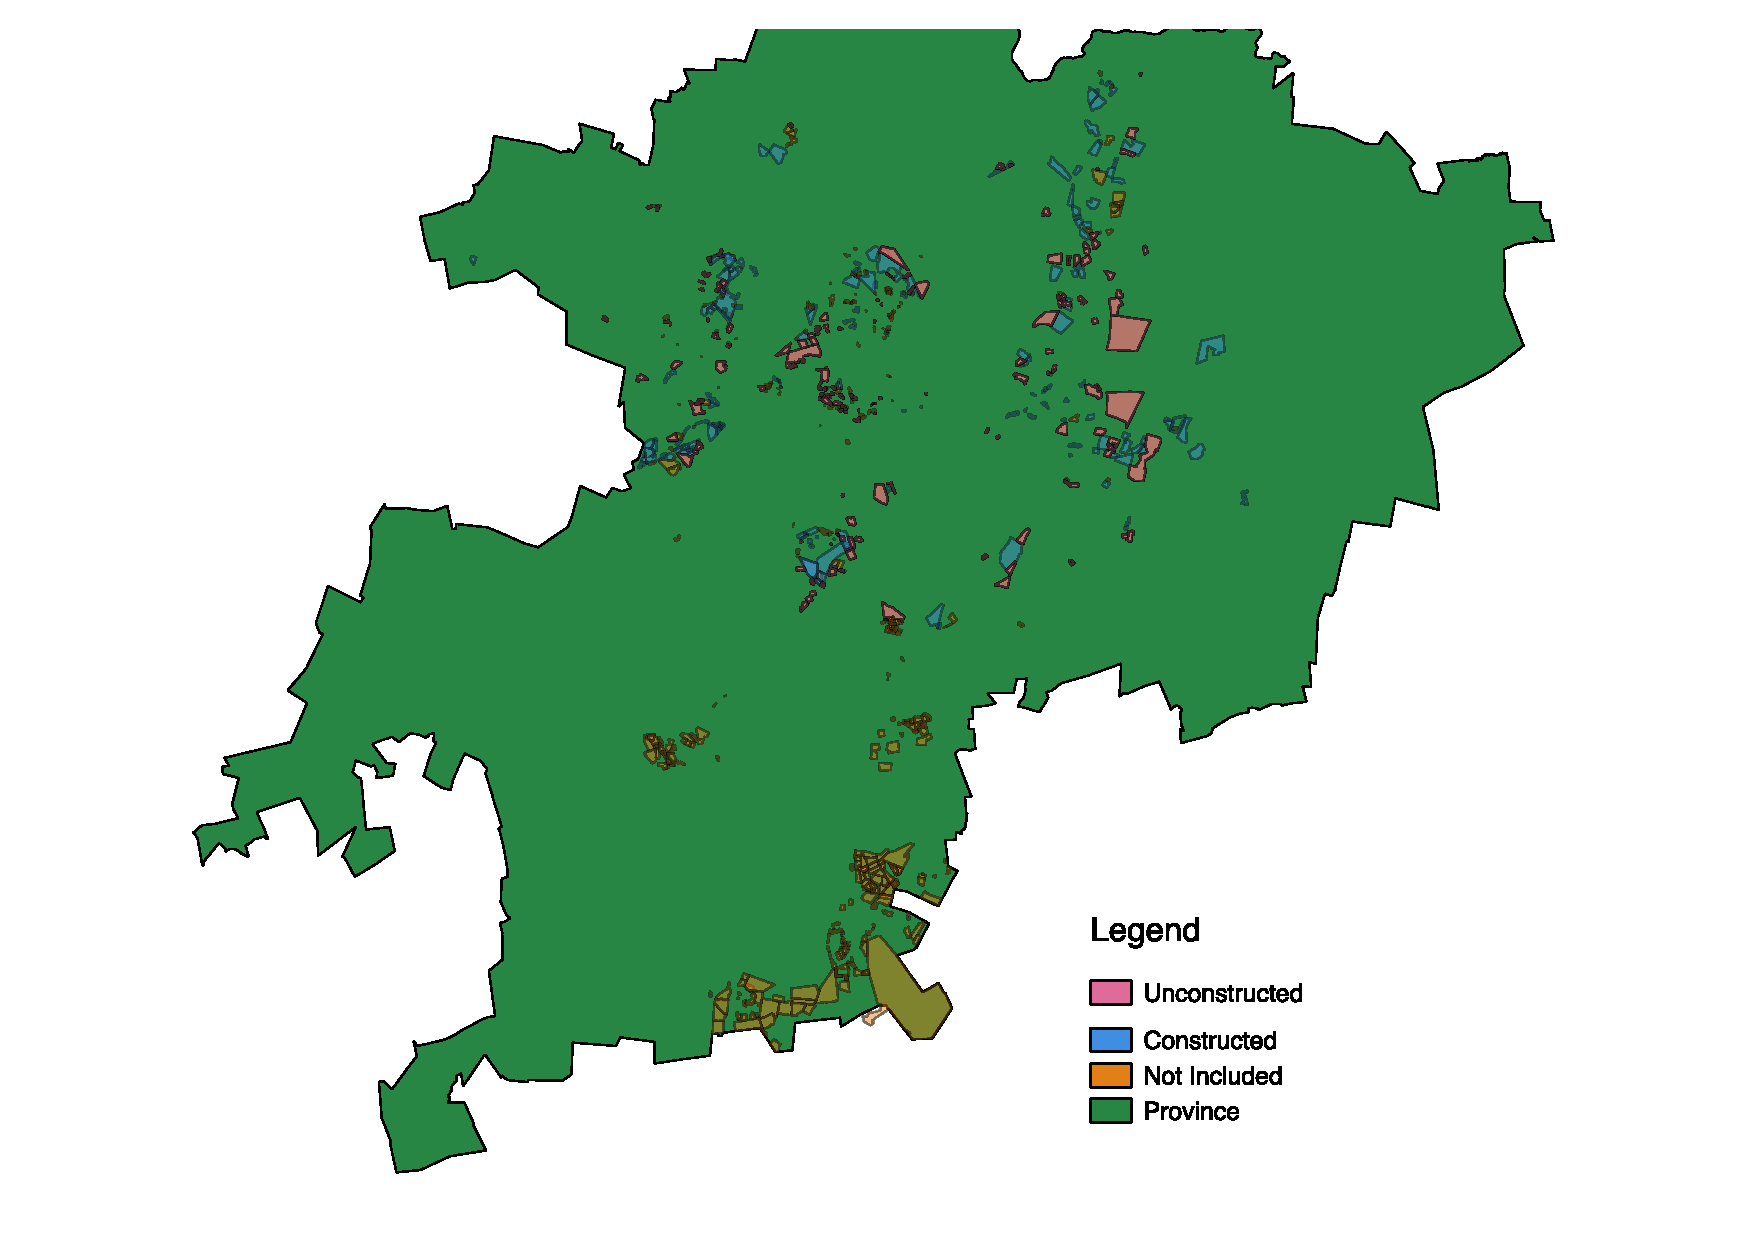
\includegraphics[scale=.7,angle=180,origin=c]{new_map.pdf}
\end{center}
\begin{itemize}
\item Pink : Unconstructed
\item Blue : Constructed
\item Orange : Not included (unclassified) 
\end{itemize}
\end{figure}


\end{document}


